
\chapter{Evaluación y Resultados}

\label{chap6:evaluacion}

\section{Introducción}

En el ámbito de investigación y desarrollo de sistemas \abbr{HAR}
existen dos elementos vitales: la recolección de datos experimentales
y generación del conjunto de entrenamiento. En este capítulo, describimos
de manera general estos elementos en las primeras dos secciones. La
sección \ref{sec6:recoleccion} describe los aspectos relacionados
a la captura de datos, determinando los requisitos mínimos de los
teléfonos móviles utilizados y describiendo el procedimiento guía
para experimentación. Posteriormente, la sección \ref{sec6:clasificacion}
describe los resultados obtenidos al aplicar las técnicas descritas
en la \secref{sec44:proceso-señales} para transformar datos sensoriales
a un conjunto de entrenamiento necesario para clasificar actividades
humanas. Esto incluye la validación del clasificador construido con
las técnicas de \emph{Machine Learning} (\abbr{ML}) expuestas en
este trabajo y confirma su efectividad en ambientes productivos. 

Finalmente, en la sección \ref{sec6:resultados} los resultados producidos
al utilizar el clasificador construido con el conjunto entrenamiento
inicial son presentados. Aquí se expone la evaluación de los resultados
producidos por \emph{HARDroid }en conjunción con la aplicación \emph{ActivitySurvey}
desarrollada para esta tarea.

\section{Datos Experimentales}

\label{sec6:recoleccion}En base a trabajos precedentes en sistemas
\abbr{HAR}, se han dispuesto datos experimentales para entrenar clasificadores
de actividades humanas tales como en \cite{ReyesOrtiz2013}. Estos
datos están disponibles para ser utilizados como fuente para diversos
estudios de investigación en este ámbito. 

Sin embargo, los datos de sensores capturados con teléfonos móviles
aún son escasos. Es por esta razón que en este trabajo se requirió
realizar una recolección acorde a los objetivos de estudio del mismo.
El procedimiento y los datos recolectados por medio de experimentación
se describen a continuación.

\subsection{Instrumentación}

Como está constatado en capítulos anteriores el desarrollo de \emph{HARDroid
}se concreto completamente para la plataforma \emph{Android }y a continuación
se detallan los rasgos técnicos de las herramientas utilizadas para
su concepción y evaluación.

\subsubsection{Teléfonos inteligentes}

Escoger las herramientas apropiadas para desarrollar un sistema \abbr{HAR}
requiere primeramente de la elección de teléfonos móviles modernos
disponibles en el mercado, teniendo en cuenta los criterios citados
en la \secref{sec24:dispositivos-moviles} en cuanto a: \emph{hardware},
sensores y plataforma de \emph{software}. En el periodo de pruebas
de este trabajo (2016), la cantidad de teléfonos inteligentes con
sensores de aceleración fue vasta, algunos de los cuales se listan
en la \tabref{tab6:dispositivos} junto con sus características relevantes.

\begin{table}[h]
\begin{centering}
\begin{tabular}{|l|>{\raggedright}p{2.5cm}|l|>{\raggedright}p{2cm}|l|}
\hline 
Marca/modelo & CPU & RAM/ROM & Sensor & Android\tabularnewline
\hline 
\hline 
LG G2 & 1.2GHz Cortex-A7 & 1GB/8GB & BMI160 & Nougat 7.0\tabularnewline
\hline 
LG Nexus 5X & Q1.4Ghz Cortex-A53 & 2GB/32GB & BMC150 & Lollipop 5.0.2\tabularnewline
\hline 
Motorola G 2nd & 1.2GHz Cortex-A7 & 1GB/8GB & 3-axis Acc & Marshmallow 6.0\tabularnewline
\hline 
Huawei Mate 9 & Q2.4GHz Cortex-A73 & 4GB/64GB & LSM6DSM & Nougat 7.0\tabularnewline
\hline 
Huawei Mate 8 & Q2.3GHz Cortex-A72 & 3GB/32GB & LSM330  & Marshmallow 6.0\tabularnewline
\hline 
Samsung S6 & Q2.1GHz Cortex-A57 & 3GB/32GB & MPU6500 & Nougat 7.0\tabularnewline
\hline 
Samsung A5 & Q1.2GHz Cortex-A53  & 2GB/16GB & BOSCH & Lollipop 5.1.1\tabularnewline
\hline 
\end{tabular}
\par\end{centering}
\caption[Especificaciones de teléfonos inteligentes]{\label{tab6:dispositivos}Especificaciones de los teléfonos inteligentes
de entrenamiento.}
\end{table}

La elección se dio en base a los teléfonos inteligentes disponibles
que fueron propiedad de los voluntarios durante las diferentes sesiones
de experimentación.

\subsubsection{Entorno de desarrollo }

Las aplicaciones móviles desarrolladas en este trabajo están enteramente
construidas para la plataforma \emph{Android}, donde fueron utilizados
los siguientes programas destinados para el caso \cite{Android2016}:
\begin{itemize}
\item \emph{Android Studio}: Entorno de desarrollo integrado para proyectos\emph{
}de software.
\item \emph{Android} \emph{Software Development Kit }(\abbr{SDK}): Herramientas
y librerías \abbr{API} requeridas para construir aplicaciones \emph{Android}.
\item \emph{Gradle}: Programa de automatización de tareas de construcción
de aplicaciones.
\end{itemize}
Las aplicaciones móviles fueron desarrolladas utilizando el lenguaje
\emph{Java}. Esto incluye las interfaces de usuario, los servicios
de aplicación, las tareas de computación intensivas de acceso a sensores,
procesamiento, algoritmos de \abbr{ML} y almacenamiento de datos
fueron desarrollados integramente en \emph{Java}.

\subsection{Procedimiento Guía }

Con el objetivo de obtener un conjunto de datos adecuado a los objetivos
estudio de sistemas \abbr{HAR} de este trabajo, se realizó un experimento
de recolección con grupo de voluntarios. Un grupo de 8 personas entre
las edades de 20 y 38 estuvieron dispuestos para esta tarea, la edad
media de la población esta comprendida en $30.7\pm5$ años. 

El procedimiento guía de captura de datos se instruyó con el uso del
teléfono móvil como prenda sujeta al bolsillo o en la cintura mientras
se realiza una actividad física predeterminada. El planeamiento del
experimento consitió en realizar en orden por un periodo de 2 a 15
minutos alguna de las tres actividades básicas y dos de transporte.
De acuerdo a la \secref{ssec44:labeling} se listan en la \tabref{tab6:etiquetas}
las actividades humanas con sus etiquetas correspondientes.

\begin{table}[h]
\begin{centering}
\begin{tabular}[t]{|c|l|l|}
\hline 
Símbolo & Etiqueta & Descripción\tabularnewline
\hline 
\hline 
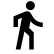
\includegraphics[scale=0.5]{capitulo-6/graphics/ic_activity_walk} & \texttt{WALKING} & Caminar\tabularnewline
\hline 
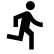
\includegraphics[scale=0.5]{capitulo-6/graphics/ic_activity_run} & \texttt{RUNNING} & Trotar\tabularnewline
\hline 
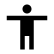
\includegraphics[scale=0.5]{capitulo-6/graphics/ic_activity_still} & \texttt{STILL} & Estar quieto\tabularnewline
\hline 
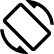
\includegraphics[scale=0.5]{capitulo-6/graphics/ic_activity_tilt} & \texttt{TILTING} & Estar inquieto\tabularnewline
\hline 
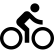
\includegraphics[scale=0.5]{capitulo-6/graphics/ic_activity_bike} & \texttt{ON\_BICYCLE } & Andar en bicicleta\tabularnewline
\hline 
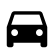
\includegraphics[scale=0.5]{capitulo-6/graphics/ic_activity_car} & \texttt{IN\_VEHICLE } & Andar en automóvil\tabularnewline
\hline 
\end{tabular}
\par\end{centering}
\caption{\label{tab6:etiquetas}Actividades humanas etiquetadas}
\end{table}

El resultado de este experimento de recolección se resume en la \tabref{tab6:sesiones},
aquí se incluyen las sesiones hechas por los voluntarios y el tiempo
en minutos acumulado que fue invertido en cada actividad. 

\begin{table}[h]
\begin{centering}
\begin{tabular}{|c|c|c|c|c|c|c|}
\hline 
\multirow{2}{*}{Individuo} & \multicolumn{6}{c|}{Actividades}\tabularnewline
\cline{2-7} 
 & \texttt{\footnotesize{}WALKING} & \texttt{\footnotesize{}RUNNING} & \texttt{\footnotesize{}STILL} & \texttt{\footnotesize{}TILTING} & \texttt{\footnotesize{}ON\_BICYLE} & \texttt{\footnotesize{}IN\_VEHICLE}\tabularnewline
\hline 
\hline 
AG & 80 & 33 & 12 & 10 & 17 & 7\tabularnewline
\hline 
SG & 15 & 15 & - & - & - & -\tabularnewline
\hline 
SF & 43 & 25 & - & - & 13 & -\tabularnewline
\hline 
GA & 30 & 2 & - & - & - & -\tabularnewline
\hline 
BV & - & 17 & - & - & - & -\tabularnewline
\hline 
PV & 17 & 19 & 12 & - & - & 7\tabularnewline
\hline 
SY & 37 & 13 &  & 10 & 26 & 11\tabularnewline
\hline 
MD & 29 & 4 & - & - & - & -\tabularnewline
\hline 
\end{tabular}
\par\end{centering}
\caption{\label{tab6:sesiones}Resumen de sesiones de entrenamiento}
\end{table}


\subsection{Captura de Datos}

Construir un clasificador requiere de una cantidad de datos recolectados
de los voluntarios mientras realizan las actividades humanas dictadas
durante el experimento. Para la captura y persistencia de las señales
del sensor de aceleración se utilizó una aplicación móvil para \emph{Android
}denominada \emph{SensorLog} \cite{Alan2014s}, este se ve en la \figref{fig4:sensor-log}.
Esta aplicación permite exportar las señales sensoriales almacenadas
en forma agrupada por sesiones y subirlas a la nube. En la \tabref{tab6:captura}
se resumen las medidas de señales capturadas durante el experimento.

\begin{table}[h]
\begin{centering}
\begin{tabular}{|c|c|c|c|c|c|}
\hline 
\multicolumn{6}{|c|}{Actividades}\tabularnewline
\hline 
\texttt{\footnotesize{}WALKING} & \texttt{\footnotesize{}RUNNING} & \texttt{\footnotesize{}STILL} & \texttt{\footnotesize{}TILTING} & \texttt{\footnotesize{}ON\_BICYLE} & \texttt{\footnotesize{}IN\_VEHICLE}\tabularnewline
\hline 
\hline 
3.591.788 & 1.604.270 & 387.735 & 134.566 & 819.992 & 365.814\tabularnewline
\hline 
\end{tabular}
\par\end{centering}
\caption{\label{tab6:captura}Unidades de datos capturados}
\end{table}


\subsection{Conjunto de Entrenamiento }

Los datos recolectados en bruto son procesadas de acuerdo al proceso
descrito en la \secref{ssec44:extraction} para formar un conjunto
de entrenamiento. En la \tabref{tab6:muestras} se resumen las muestras
obtenidas al aplicar las técnicas de procesamiento de datos de este
trabajo. 

\begin{table}[h]
\begin{centering}
\begin{tabular}{|c|c|c|c|c|c|}
\hline 
\multicolumn{6}{|c|}{Actividades}\tabularnewline
\hline 
\texttt{\footnotesize{}WALKING} & \texttt{\footnotesize{}RUNNING} & \texttt{\footnotesize{}STILL} & \texttt{\footnotesize{}TILTING} & \texttt{\footnotesize{}ON\_BICYLE} & \texttt{\footnotesize{}IN\_VEHICLE}\tabularnewline
\hline 
\hline 
5.915 & 3.019 & 645 & 485 & 1.338 & 610\tabularnewline
\hline 
\end{tabular}
\par\end{centering}
\caption{\label{tab6:muestras}Unidades de muestras procesadas}
\end{table}

La generación del clasificador de \abbr{ML} de este trabajo está
automatizado por medio una herramienta construida en \emph{Java. }El
proceso se puede apreciar en el siguiente flujo de la \figref{fig6:proceso-clasi}.

\begin{figure}[th]
\begin{centering}
\includegraphics[width=0.8\textwidth]{\string"capitulo-6/graphics/Proceso de Clasificacion\string".png}
\par\end{centering}
\caption{\label{fig6:proceso-clasi}Flujo de generación del clasificador C4.5}
\end{figure}

Las entradas iniciales son los archivos de datos \emph{Sensor TS i},
donde $i=1,..,N$ dependiendo de la cantidad de voluntarios. El procesamiento
de \emph{Cálculo Features} produce un conjunto de entrenamiento \emph{Features
TS }que forma el modelo inicial del \emph{Clasificador C4.5} para
producir un \emph{Decision tree} que es empaquetado en una librería
\emph{Java}.

\section{Clasificador de Actividades Humanas}

\label{sec6:clasificacion}El clasificador de reconocimiento de actividades
humanas (\abbr{HAR}) construido en este trabajo es un clasificador
de clases discretas que utiliza un algoritmo de aprendizaje automático
supervisado basado en árboles de decisión. 

En esta sección se describe el procedimiento de generación de un clasificador
\abbr{HAR} utilizando el conjunto de entrenamiento inicial descrito
en la sección anterior. El clasificador es evaluado por medio de pruebas
y verificación que puedan garantizar su efectividad. El procedimiento
de construcción se realiza con la herramienta de \abbr{ML} denominada
\emph{Waikato Environment Knowledge Analysis} \texttt{(\abbr{WEKA})}
\cite{Frank2016}.

El clasificador es un árbol de decisión obtenido por medio del algoritmo
C4.5 (\algref{algoC45}) y la implementación en \emph{Java} J48 \cite{Frank2016b}
considerando los siguientes parámetros:
\begin{itemize}
\item Umbral de confianza para poda\emph{ }(-C\emph{ confidenceFactor}):
$0.25$
\item Numero mínimo de instancias permisibles por hoja\emph{ }(-M\emph{
minNumObj}): $2$
\item Tamaño del conjunto de poda\emph{ }(-N\emph{ numFolds}): $3$
\item Pliegue de Validación Cruzada\emph{ }(\emph{Cross-validation folds}):
$10$
\end{itemize}

\subsection{Métricas de predicción }

\label{ssec6:metricas}De manera a evaluar el rendimiento de los clasificadores
de aprendizaje automático supervisado se describen las siguientes
medidas y métricas numéricas de predicción que dan una noción de cuánto
se acercan a los datos observados \cite{Witten2017}. Con la utilización
de la validación cruzada por estratos de diez (\emph{10-fold}) resulta
en las siguientes medidas:
\begin{itemize}
\item \emph{Número de instancias} ($N$): es el tamaño de la población de
entrada.
\item \emph{Instancias correctamente clasificadas} ($C$): es una proporción
del tamaño de la población de entrada.
\item \emph{Instancias incorrectamente clasificadas} \emph{(}$I$): es un
proporción del tamaño de la población de entrada.
\item \emph{Estadísticas Kappa} ($\kappa$): es el coeficiente \emph{kappa}
de \emph{Cohen} que determina el valor de coeficiente de concordancia
para confiabilidad de los datos según los rangos de la \tabref{tab6:kappa-coef}
y se obtienen con la ecuación: 
\[
\kappa\text{=}\frac{p_{o}-p_{e}}{1-p_{e}}
\]
Donde $p_{o}$ es el acuerdo observado relativo y $p_{e}$ es la probabilidad
hipotética de acuerdo.
\end{itemize}
\begin{table}[h]
\begin{centering}
\begin{tabular}{|c|c|c|}
\hline 
Valor & Nivel de acuerdo & \% de datos confiables\tabularnewline
\hline 
\hline 
0 - 0.20 & No & 0 - 4\%\tabularnewline
\hline 
0.21 - 0.39 & Mínimo & 4 - 15\%\tabularnewline
\hline 
0.40 - 0.59 & Débil & 15 - 35\%\tabularnewline
\hline 
0.60 - 0.79 & Moderado & 35 - 63\%\tabularnewline
\hline 
0.80 - 0.90 & Fuerte & 64 - 81\%\tabularnewline
\hline 
>0.90 & Casi perfecto & 82 - 100\%\tabularnewline
\hline 
\end{tabular}
\par\end{centering}
\caption{\label{tab6:kappa-coef}Rango de valores de coeficiente$\kappa$}
\end{table}

En un problema de clasificación de datos desconocidos a partir de
una cantidad de datos de entrada limitados, la técnica de validación
cruzada dan una idea de la capacidad de un algoritmo al clasificar
instancias de prueba con cierta precisión. 

También es importante conocer el costo asociado de una clasificación
no acertada en términos del error. Si el clasificador predice una
clase como: correcta es tenida en cuenta como éxito, sino es un error.
Por lo tanto, la razón de error es solo una proporción de errores
hecho sobre el conjunto total de instancias y mide el rendimiento
de clasificador. 

Por otra parte, existen otras métricas numéricas útiles para evaluar
la predicción en base a los errores. De acuerdo a la nomenclatura
presentada en la \secref{sec3:aprendizaje}, definición \ref{def3:clasificacion}
donde se considera a $f(x_{i})$ como el valor pronosticado de una
instancia de evaluación $x_{i}$ dada, e $y_{i}$ corresponde al valor
real de esta \emph{$i$-ésima} instancia, se tiene cuanto sigue \cite{Witten2017}:
\begin{itemize}
\item \emph{Error medio absoluto}: es el promedio de los errores absolutos
individuales.
\[
E_{ma}=\frac{1}{n}\sum_{i\text{=1}}^{n}\bigl|y_{i}-f(x_{i})\bigr|
\]
Está medida no exagera el efecto de los valores atípicos (\emph{outliders}),
todos los errores son tratados de igual conforme a su magnitud.
\item \emph{Raíz de Error cuadrático medio}: es la raíz del promedio de
los errores cuadráticos individuales.
\[
E_{rms}=\sqrt{\frac{1}{n}\sum_{i\text{=1}}^{n}\left(y_{i}-f(x_{i})\right)^{2}}
\]
Es una medida de fácil manipulación matemática con la misma dimensión
que el valor pronosticado y además comúnmente utilizada en técnicas
de regresión lineal aunque tiende a exagerar el efecto de los valores
atípicos.
\item \emph{Error absoluto relativo}: es la suma de los errores absolutos
relativo a la suma de errores absolutos respecto a la media.
\[
E_{ra}=\sum_{i\text{=1}}^{n}\frac{\bigl|y_{i}-f(x_{i})\bigr|}{\bigl|y_{i}-\bar{y}\bigr|}\,\textrm{, donde\,}\bar{y}=\frac{1}{n}\sum_{i=1}^{n}y_{i}
\]
Representa el error total absoluto normalizado con el error absoluto
respecto a un predictor simple como lo es el promedio de valores reales.
\item \emph{Raíz de Error cuadrático relativo}: es la raíz de la suma de
los errores cuadráticos individuales relativo a la suma de los errores
cuadráticos respecto a la media. 
\[
E_{rrs}=\sqrt{\sum_{i\text{=1}}^{n}\frac{\left(y_{i}-f(x_{i})\right)^{2}}{\left(y_{i}-\bar{y_{i}}\right)^{2}}}
\]
Representa el error total cuadrático normalizado con el error cuadrático
respecto a un predictor simple como lo es el promedio de valores reales.
\end{itemize}
Escoger cuales de estas métricas son apropiadas para una evaluación
dependen mucho del estudio y de la aplicación del aprendizaje automático.
Por ejemplo, si se trata de minimizar alguna métrica o disminuir el
costo asociado a un error en particular. En general, sobre los errores
cuadráticos y/o la raíz de los mismos pesan mas las grandes discrepancias
que las pequeñas, mientras que en errores absolutos no. Los errores
relativos tratan de compensar la predictabilidad del valor pronosticado,
tratando siempre de tender hacia el valor real medio. 

\subsection{Evaluación del clasificador}

El clasificador generado en este trabajo es un árbol de decisión de
tamaño de $677$ nodos, de los cuales $339$ corresponden a hojas.
Las métricas numéricas de predicción se exponen a continuación considerando
las muestras de entrenamiento descritas anteriormente: 
\begin{itemize}
\item Número de instancias ($N$): $12.012$ 
\item Instancias correctamente clasificadas ($C$): $10.942$ ($91,0922\%$)
\item Instancias incorrectamente clasificadas ($I$): $1.070$ ($8,9078\%$)
\item Estadísticas Kappa ($\kappa$): $0,8678$ 
\item Error medio absoluto ($E_{ma}$): $0,0341$
\item Raíz de Error cuadrático medio ($E_{rms}$): $0,164$ 
\item Error absoluto relativo ($E_{ra}$): $15,1717\%$ 
\item Raíz de Error cuadrático relativo ($E_{rrs}$): $48,9126\%$ 
\end{itemize}
La discusión que surge de estos cálculos es que para el conjunto de
entrenamiento de $12.012$ instancias el clasificador tiene una taza
de predicción del $91,1\%$ de las veces correctamente y el $8,9\%$
de las veces incorrectamente. El valor del coeficiente de confianza
está entre el $0,8-0,9$ dando un porcentaje aproximado de $74,6%\%
$ considerado como una fuerte confianza en los datos.

En cuanto a los errores, se puede observar que el error absoluto es
bajo y el error cuadrático es bajo moderado ya que son menos que un
$20\%$. Los errores relativos con respecto al error simple utilizando
la media arrojan un valor moderado de $15,2\%$ para el absoluto y
un valor medio de $48,9\%$ para el cuadrático. 

Estos errores dan una noción del costo de la predicción, un incremento
en el error a partir de una situación inicial, sin importar cual sea
la métrica, implica inherentemente una situación inicial de mayor
variabilidad y de difícil de predicción, no que el clasificador es
peor.

Además, utilizando la técnica de validación cruzada explicada en la
\secref{sec3:metricas} se obtiene la matriz de confusión resultante
en la \tabref{tab6:matriz-confusion}. 

\begin{table}[h]
\begin{centering}
\begin{tabular}{|l|c|c|c|c|c|c|}
\cline{2-7} 
\multicolumn{1}{l|}{} & \multicolumn{6}{c|}{Matriz de Confusión}\tabularnewline
\hline 
Actividad & \texttt{\footnotesize{}WALKING} & \texttt{\footnotesize{}RUNNING} & \texttt{\footnotesize{}STILL} & \texttt{\footnotesize{}TILTING} & \texttt{\footnotesize{}ON\_BICYLE} & \texttt{\footnotesize{}IN\_VEHICLE}\tabularnewline
\hline 
\hline 
\texttt{\footnotesize{}WALKING} & \textbf{5.643} & 63 & 21 & 28 & 156 & 4\tabularnewline
\hline 
\texttt{\footnotesize{}RUNNING} & 122 & \textbf{2.852} & 3 & 6 & 36 & 0\tabularnewline
\hline 
\texttt{\footnotesize{}STILL} & 19 & 14 & \textbf{555} & 23 & 15 & 19\tabularnewline
\hline 
\texttt{\footnotesize{}TILTING} & 26 & 3 & 21 & \textbf{304} & 46 & 85\tabularnewline
\hline 
\texttt{\footnotesize{}ON BICYLE} & 157 & 28 & 7 & 47 & \textbf{1.089} & 10\tabularnewline
\hline 
\texttt{\footnotesize{}IN VEHICLE} & 2 & 2 & 14 & 86 & 7 & \textbf{499}\tabularnewline
\hline 
\end{tabular}
\par\end{centering}
\caption{\label{tab6:matriz-confusion}Matriz de confusión del clasificador
generado}
\end{table}

Con esta matriz se calculan las siguientes métricas de evaluación
para clasificadores descritas en la \secref{sec3:metricas}:
\begin{itemize}
\item Precisión: $0,9174$
\item Exhaustividad: $0,9109$
\item Exactitud: $0,9714$
\item \emph{Valor-F}: $0,9142$
\end{itemize}
Estos valores arrojan una perspectiva de que el clasificador generado
posee altos valores de exactitud, precisión y exhaustividad. Esto
se corresponde por la baja tasa de falsos positivos y negativos. En
cuanto al \emph{Valor-F}, el valor del mismo es alto en proporción
a los valores de precisión y exhaustividad, ya que es de forma general
la media armónica de ambos.

\section{Resultados Experimentales}

\label{sec6:resultados}En esta sección se describen los resultados
del experimento realizado utilizando la aplicación \emph{ActivitySurvey}
que utiliza el reconocedor \emph{HARDroid}, ambos desarrollados en
este trabajo. Los datos presentados en esta sección permiten verificar
el funcionamiento correcto de los componentes de software implementados
así como también validar las predicciones emitidas por el reconocedor
de actividades humanas contribuido en este trabajo.

\subsection{Verificación del Clasificador HAR}

Para verificar el clasificador \abbr{HAR} de \emph{HARDroid }se condujo
un experimento de prueba basado en una sesión de actividades físicas
realizadas por dos personas. El protocolo consitió en realizar cada
una de las actividades básicas ambulatorias y de transporte por un
periodo comprendido entre 10 a 20 minutos utilizando la aplicación
\emph{ActivitySurvey}. 

En la \tabref{tab6:vsesiones} se muestra el resumen del tiempo invertido
en minutos por cada persona en las actividades humanas realizadas
en una sesión de evaluación de una hora aproximadamente.

\begin{table}[th]
\begin{centering}
\begin{tabular}{|c|c|c|c|c|c|c|}
\hline 
\multirow{2}{*}{Teléfono} & \multicolumn{6}{c|}{Actividades}\tabularnewline
\cline{2-7} 
 & \texttt{\footnotesize{}WALKING} & \texttt{\footnotesize{}RUNNING} & \texttt{\footnotesize{}STILL} & \texttt{\footnotesize{}TILTING} & \texttt{\footnotesize{}ON\_BICYLE} & \texttt{\footnotesize{}IN\_VEHICLE}\tabularnewline
\hline 
\hline 
nexus5x & 14 & 10 & 10 & - & 20 & 14\tabularnewline
\hline 
mate9 & 12 & 7 & 18 & - & 15 & 14\tabularnewline
\hline 
\end{tabular}
\par\end{centering}
\caption{\label{tab6:vsesiones}Resumen de sesiones de evaluación}
\end{table}

La aplicación móvil \emph{ActivitySurvey} consulta la actividad humana
detectada al servicio autónomo \emph{HARDroid} en intervalos regulares.
Durante una sesión se registra la información del teléfono, correo,
edad, la fecha y hora, la etiqueta de la actividad detectada y la
etiqueta de la actividad corregida en caso de una aseveración. 

En la \tabref{tab6:vencuesta} se muestra las cantidades de las actividades
acertadas y no acertadas por el clasificador \abbr{HAR} en proporción
con el total de detecciones recolectadas durante las encuestas realizadas
en cada sesión. Una respuesta de desacierto coincide con una etiqueta
obtenida por retroalimentación del usuario.

\begin{table}[h]
\begin{centering}
\begin{tabular}{|l|c|c|c|c|c|c|}
\cline{2-5} 
\multicolumn{1}{l|}{} & \multicolumn{4}{c|}{\textbf{Desaciertos}} & \multicolumn{1}{c}{} & \multicolumn{1}{c}{}\tabularnewline
\hline 
Actividad & \texttt{\footnotesize{}WALKING} & \texttt{\footnotesize{}STILL} & \texttt{\footnotesize{}ON\_BICYLE} & \texttt{\footnotesize{}IN\_VEHICLE} & \textbf{\small{}Aciertos} & \textbf{\small{}Porcentaje}\tabularnewline
\hline 
\hline 
\texttt{\footnotesize{}WALKING} &  &  & 13 &  & 151 & 92,07\%\tabularnewline
\hline 
\texttt{\footnotesize{}RUNNING} &  &  & 13 &  & 83 & 86,46\%\tabularnewline
\hline 
\texttt{\footnotesize{}STILL} &  &  &  & 8 & 140 & 94,59\%\tabularnewline
\hline 
\texttt{\footnotesize{}TILTING}\emph{\footnotesize{}}\footnote{{\footnotesize{}Estar inquieto no se considera una actividad ambulatoria,
presentándose los datos de manera informativa}} &  &  &  & 38 & 0 & 0,00\%\tabularnewline
\hline 
\texttt{\footnotesize{}ON\_BICYLE} & 8 &  &  & 4 & 59 & 83,10\%\tabularnewline
\hline 
\texttt{\footnotesize{}IN\_VEHICLE} &  & 11 &  &  & 83 & 88,30\%\tabularnewline
\hline 
\end{tabular}
\par\end{centering}
\caption[Aciertos y desaciertos de actividades humanas detectadas]{\label{tab6:vencuesta}Resumen de actividades detectadas marcadas
como aciertos o desaciertos}
\end{table}

Según estos resultados se puede concluir que con un promedio de $88.9%\%
$ de aciertos el clasificador tiene una alta taza de aciertos la mayoría
de las actividades humanas evaluadas, específicamente las actividades
en bicicleta y en vehículo son las que más poseen falsos negativos.

\subsection{Validación de la Clasificación}

Para validar los resultados de la clasificación producida por \emph{HARDroid
}se condujo un experimento de prueba basado en la misma sesión de
actividades físicas realizadas por una persona. El protocolo consitió
en utilizar la aplicación \emph{Sony} \emph{Lifelog} al mismo tiempo
que la aplicación \emph{ActivitySurvey} durante las sesiones de pruebas. 

En la \tabref{tab6:vclasificacion} se muestra el intervalo de tiempo
de la sesión y su duración para cada actividad humana realizada por
una persona.

\begin{table}[h]
\begin{centering}
\begin{tabular}{|c|>{\raggedright}p{3cm}|c|c|>{\raggedright}p{3cm}|c|}
\hline 
Teléfono & Etiqueta 

\emph{Sony Lifelog} & Intervalo & Duración & Etiqueta \emph{HARDroid} & Relación\tabularnewline
\hline 
\hline 
nexus5x & \texttt{walking} & 21:26 - 21:44 & 19 & \texttt{WALKING} & 45/9\tabularnewline
\hline 
nexus5x & \texttt{cycling} & 21:44 - 22:00 & 27 & \texttt{ON\_BICYCLE} & 32/8\tabularnewline
\hline 
nexus5x & \texttt{running} & 22:12 - 22:24 & 13 & \texttt{RUNNING} & 41/0\tabularnewline
\hline 
nexus5x & \texttt{vehicle} & 22:39 - 22:57 & 19 & \texttt{IN\_VEHICLE} & 32/6\tabularnewline
\hline 
nexus5x & \texttt{-} & 22:25 - 22:35 & 10 & \texttt{STILL} & 65/0\tabularnewline
\hline 
\end{tabular}
\par\end{centering}
\caption[Evaluación \emph{HARDroid} vs \emph{Sony LifeLog}]{\label{tab6:vclasificacion}Comparación de actividades detectadas
por \emph{HARDroid} vs\emph{ Sony Lifelog}}
\end{table}

Cada actividad detectada por \emph{HARDroid} fue validada con la aplicación
\emph{Sony} \emph{Lifelog} cuyo acierto se considera del 100\% en
comparación con la relación de aciertos y desaciertos extraidos de
los resultados de la sección anterior para una persona en particular. 

En la \figref{fig6:vlifelog} se muestran dos pantallas de la aplicación
\emph{Sony Lifelog }capturadas durante las sesiones de prueba donde
se confirma como veracidad las actividades físicas realizadas durante
el intervalo de cada sesión.

\begin{figure}[th]
\begin{centering}
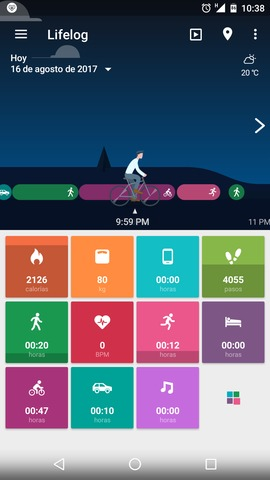
\includegraphics[scale=0.6]{capitulo-6/graphics/lifelog1} 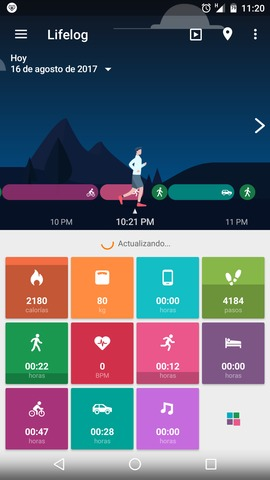
\includegraphics[scale=0.6]{capitulo-6/graphics/lifelog2}
\par\end{centering}
\caption[Actividades reconocidas con \emph{Sony Lifelog}]{\label{fig6:vlifelog}Actividades físicas capturadas con la aplicación
\emph{Sony Lifelog}}
\end{figure}

La aplicación \emph{Sony Lifelog} representa las actividades físicas
por símbolos visuales similares a la \tabref{tab6:etiquetas}, donde
se pueden apreciar las actividades realizadas de: caminata, trote,
en bicicleta y en automóvil.

\subsection{Entrenamiento Colaborativo}

Así como se expuso en la \secref{sec55:activity}, la aplicación móvil
\emph{ActivitySurvey} está diseñada para recabar información que pueda
ser utilizada para mejorar el clasificador continuamente. Utilizando
este enfoque la información recolectada durante la evaluación fue
combinada con los datos calculados inicialmente para generar un nuevo
clasificador con datos colaborados durante las pruebas.

Siguiendo el mismo procedimiento de la \secref{sec6:clasificacion}
se generó un clasificador colaborativo, a partir de las instancias
aseveradas como aciertos, y se obtuvo un árbol de decisión de tamaño
de $699$ nodos, de los cuales $350$ corresponden a hojas. Las métricas
de evaluación para clasificadores descritas en la \secref{sec3:metricas}
son:
\begin{itemize}
\item Precisión: $0,9204$
\item Exhaustividad: $0,9134$
\item Exactitud: $0,9723$
\item \emph{Valor-F}: $0,9168$
\end{itemize}
Los valores aumentan levemente en comparación con el clasificador
inicial. En cuanto a las métricas numéricas se muestran en la \tabref{tab6:comparacion-clasi}
en comparación con el clasificador inicial de forma resumida con su
símbolo correspondiente.

\begin{table}[H]
\begin{centering}
\begin{tabular}{|c|c|c|}
\hline 
Métrica & Inicial & Colaborativo\tabularnewline
\hline 
\hline 
$N$ & 12.012 & 12.578\tabularnewline
\hline 
$C$ & 10.942 (91,09\%) & 11.489 (91,34\%)\tabularnewline
\hline 
$I$ & 1.070 (8,91\%) & 1.089 (8,66\%)\tabularnewline
\hline 
$\kappa$ & 0,8678 & 0,8735\tabularnewline
\hline 
$E_{ma}$ & 0,0341 & 0,0333\tabularnewline
\hline 
$E_{rms}$ & 0,164 & 0,1632\tabularnewline
\hline 
$E_{ra}$ & 15,17\% & 14,58\%\tabularnewline
\hline 
$E_{rrs}$ & 48,91\% & 48,30\%\tabularnewline
\hline 
\end{tabular}
\par\end{centering}
\caption{\label{tab6:comparacion-clasi}Comparación entre modelo inicial y
el colaborativo}
\end{table}

De acuerdo a estos resultados se aprecia que el clasificador colaborativo
mejora levemente en comparación al inicial como es de notar el aumento
de la precisión, la taza de aciertos, el valor del coeficiente de
confianza, así también la reducción en los valores de los errores
absolutos, cuadráticos y relativos. Con estos valores numéricos podemos
resumir que un clasificador mejora de manera continua por medio de
la retroalimentación de instancias recolectadas en campo, pero teniendo
en consideración la sensibilidad que en algunos casos se puedan introducir
instancias no acertadas.
